\chapter{Descripción del Trabajo}
\label{cap:descripcionTrabajo}

\chapterquote{¡Datos! ¡Datos! ¡Datos! - exclamó con impaciencia - No puedo hacer ladrillos sin arcilla}{El misterio de Copper Beeches\\Arthur Conan Doyle (1892)}

Aquí comienza la descripción del trabajo realizado. Se deben incluir tantos capítulos como sea necesario para describir de la manera más completa posible el trabajo que se ha llevado a cabo. Como muestra la figura, está todo por hacer.

Si te sirve de utilidad,  puedes incluir tablas para mostrar resultados, tal como se ve en la tabla.

\section{Análisis de los datos}
El primer paso en todo trabajo de ciencia de datos e inteligencia artificial es el análisis de los datos con los que se cuenta para entrenar y probar el modelo. \textcolor{red}{Completar introducción}

\subsection{Enron corpus}\label{ss:enron}
Para llevar a cabo cualquier trabajo relacionado con la ciencia de datos e inteligencia artificial es necesario contar con un conjunto de datos con el que poder entrenar al modelo desarrollado. Cuando se trata de un estudio relacionado con la generación de lenguaje natural, el conjunto de datos se llama corpus y suele contener ejemplos de documentos reales redactados por humanos similares a los que se desea producir. En concreto, para este trabajo, se ha elegido el corpus conocido como Enron\footnote{\url{http://www-2.cs.cmu.edu/~enron/}}, dado que los correos electrónicos que contiene pertenecieron a la empresa con el mismo nombre. Precisamente se hicieron públicos tras una investigación legal llevada a cabo a esta compañía por parte de la Comisión Federal de Regulación de la Energía\footnote{\url{https://www.ferc.gov/}} de Estados Unidos.

Enron corpus contiene 517.401 correos electrónicos escritos en inglés de 150 usuarios distintos. Además de la ventaja de la gran cantidad de elementos pertenecientes a este dataset, también ha sido elegido por encontrar diversos trabajos sobre este mismo conjunto de e-mails, como el llevado a cabo por \cite{klimt2004introducing}.

Este corpus está organizado en una jerarquía de directorios (uno por cada usuario), en la que dentro de los principales se encuentran las correspondientes carpetas de la cuenta de correo electrónico del usuario en cuestión, como bandeja de entrada, enviados y directorios personalizados. En estas carpetas se encuentran, cada uno en un archivo separado, los distintos correos electrónicos del corpus. Un ejemplo de cómo se presentan los diferentes e-mails viene reflejado en la figura \ref{fig:emailenron}.

\begin{figure}[h]
	\centering%
	\centerline{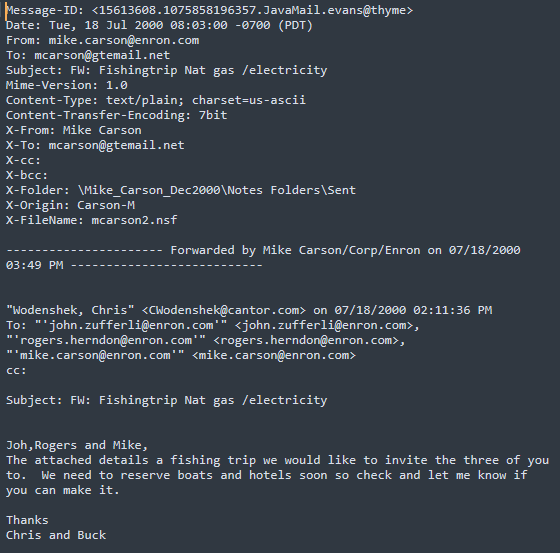
\includegraphics[width = 0.9\textwidth]{Imagenes/Bitmap/email-example.png}}%
	\caption{Ejemplo de un correo electrónico del corpus Enron}%
	\label{fig:emailenron}
\end{figure}

Como puede observarse en la figura \ref{fig:emailenron}, cada uno de los correos electrónicos se encuentra en un archivo distinto estructurado según el formato MIME explicado anteriormente (véase la sección \ref{ss:mime}). Claramente, se pueden diferenciar las distintas cabeceras de este formato con la información correspondiente a cada una de ellas. Después de todas estas cabeceras, se encuentra el cuerpo del mensaje. Por cada uno de los 517.401 correos electrónicos, se encuentra un archivo diferente con esta estructura.

\subsection{Preparación y limpieza de los datos}\label{ss:prep}

El primer problema que aparece ante el conjunto de datos elegidos es el formato en que se presentan cada uno de los correos electrónicos, ya que en cada archivo hay mucha información que generaría ruido y dificultaría el entrenamiento del modelo si no se eliminara (como las cabeceras MIME). Por ese motivo, es necesario preprocesar cada uno de ellos. Asimismo, se conseguiría un dataset apto para el propósito de construir un sistema de generación de lenguaje natural que redacte correos electrónicos.

Para extraer la información relevante de cada uno de ellos, el lenguaje de programación \textit{Python} cuenta con una librería\footnote{\url{https://docs.python.org/3/library/email.parser.html}} capaz de parsear correos electrónicos almacenados en archivos y cadenas de caracteres en formato MIME. Además, una vez procesadas las cadenas, la clase devuelta cuenta con una serie de métodos que facilitan la obtención de la información de las cabeceras y recorrer el árbol de partes MIME (véase la sección \ref{ss:mime} o consúltese el ejemplo de árbol representado en la figura \ref{fig:content-type}). De manera que solo ha sido necesario desarrollar un método que vaya recorriendo la estructura arbórea, comprobando el tipo MIME del nodo, y extrayendo el cuerpo del mensaje cuando lo encuentre.

Una vez se ha resuelto el problema de recuperar el correo electrónico dado el archivo perteneciente al corpus, es posible enfrentarse a otro reto antes del análisis exploratorio de los datos: la limpieza del cuerpo del mensaje para contar con un texto plano de cara al entrenamiento del modelo. Siempre, en todo trabajo en ciencia de datos, se presenta una fase de limpieza de los datos. Este paso resulta ligeramente más complicado cuando se está tratando con cadenas de caracteres. En el caso que ocupa a este trabajo, la limpieza consiste en encontrar patrones externos al cuerpo del mensaje, como la firma o la inclusión del mensaje al que se responde debajo de la respuesta, que no constituyen texto escrito por los usuarios, sino que ha sido incluido por el servidor de correo electrónico. Por ejemplo, en la figura \ref{fig:emailenron}, se muestra un e-mail el cual simplemente está reenviando otro mensaje distinto sin incluir más información. Esto resulta evidente por el comienzo del cuerpo del correo electrónico, que indica el reenvío. Este e-mail no debería incluirse en el entrenamiento de nuestro modelo, porque no añade información nueva y repite un mensaje que ya se tiene en otro archivo (dado que se cuenta con todos los correos del usuario, si el usuario está reenviando un e-mail, significa que es posible encontrar el mensaje original en la bandeja de entrada o alguna de las otras carpetas de su cuenta de correo). Por este motivo, es indispensable limpiar el cuerpo de los todos correos electrónicos del corpus.

Tras analizar concienzudamente el corpus de correos electrónicos se detectan varios patrones que deben abordarse y cambios que tienen que llevarse a cabo en los mensajes. El primero de ellos consiste en que, cuando un usuario contesta a un mensaje, el servidor incluye el mensaje que es respondido debajo de la contestación. En este caso solo interesa la respuesta y no el texto original (pues estará en otro archivo). No obstante, esta casuística no constituye un problema complicado de solventar, ya que se puede distinguir la respuesta del mensaje original porque siempre se incluye una cabecera de texto que no varía. Es decir, basta con encontrar la cabecera como subcadena en el cuerpo y eliminar todo lo que le preceda. La misma solución puede aplicarse al patrón que aparece cuando se envía un correo electrónico modificando una convocatoria de reunión. Resulta que el servidor genera una cabecera para diferenciar la modificación de la convocatoria original.

Ligeramente más complicado respecto a los patrones anteriores, aunque no demasiado, resulta el caso que se muestra en la figura \ref{fig:emailenron}. Se trata del reenvío de un e-mail. Cuando esto ocurre, la cabecera producida por el servidor no se trata de una subcadena fija, sino que incluye como información variable adicional el nombre del usuario que reenvía el correo, así como la fecha y hora en que se produce dicho reenvío. Aunque la solución sea la misma, eliminar lo que preceda a esta cabecera, no basta con buscar una subcadena que no varía, se requiere la utilización de expresiones regulares \citep{thompson1968programming}. Como la gran mayoría de lenguajes de programación, Python cuenta con un módulo para implementar expresiones regulares\footnote{\url{https://docs.python.org/3/library/re.html}} que ha facilitado enormemente esta tarea y ha hecho posible la limpieza de los mensajes con este patrón.

Otro problema que ha sido necesario abordar es el de la firma de los servidores de correo (frases al final de los mensajes como ``Get your FREE download of MSN Explorer''). Al ser siempre iguales, simplemente ha bastado con detectarlos y eliminar dicha subcadena del cuerpo de los mensajes. La dificultad de este tipo de limpieza de texto en realidad reside en detectar estos patrones, ya que, al tratarse de cadenas de caracteres, es complicado detectar incongruencias o errores.

Por último, debido al formato establecido por el protocolo MIME (por lo general depende de la codificación especificada para el mensaje), los servidores de correo electrónico incluyen tabulaciones y saltos de línea con una determinada frecuencia entre las palabras del texto, incluso aunque el usuario no los haya introducido. Dado que el salto de línea o la tabulación no es una información que se considere relevante de cara a la generación de texto de este modelo, se decide transformar estos caracteres en espacios y, a continuación, aplicar las expresiones regulares para detectar las subcadenas en las que se observe más de un espacio en blanco seguido y sustituirlas por uno solo.

Con esto concluye la limpieza de los cuerpos de los mensajes y la fase de preparación de los datos para adaptar los correos electrónicos a un formato adecuado para el sistema de almacenamiento elegido.

\subsection{Procesado y almacenamiento}\label{ss:almacen}

Como se ha explicado en el apartado \ref{ss:enron}, por defecto el corpus se almacena localmente estructurado en una jerarquía de directorios y contando con un archivo por cada correo electrónico. Sin embargo, esta forma de almacenamiento no resulta la más adecuada debido a que imposibilita cualquier método de búsqueda eficiente (sería necesario, en el peor de los casos, abrir todos los archivos para encontrar, por ejemplo, un e-mail en función del identificador del mensaje) y resulta excesivamente lento cuando se pretende procesar todos los mensajes (requiere recorrer la jerarquía como una estructura de datos arbórea entrando en todos los directorios). Por estas razones, la decisión de cambiar el sistema de almacenamiento es acertado para agilizar tanto la carga del corpus como las distintas operaciones que se pueden querer llevar a cabo sobre el mismo.

Como los elementos del conjunto son textos, es decir, datos no estructurados, un almacenamiento clásico en archivos de extensión \textit{.csv} podría provocar problemas como la elección del separador de los distintos campos, habría que utilizar un caracter que no apareciera en ningún cuerpo de mensaje ni en sus otras propiedades (asunto, identificador, destinatario, emisor, etcétera). Por lo tanto, un sistema relacional no parece que sea la mejor opción de almacenamiento para los correos electrónicos. Ante esta situación, se ha elegido el uso del sistema de base de datos NoSQL MongoDB (léase la sección \ref{ss:mongodb}) alojado en la nube\footnote{\url{www.mongodb.com/cloud}}. La decisión de no implantarlo en un repositorio local se sustenta sobre la ventaja que ofrece la nube de disponibilidad desde cualquier dispositivo, lo cual ha sido de gran ayuda en el proceso de desarrollo del trabajo.

Una vez se ha seleccionado la forma de almacenamiento, queda por determinar las colecciones que se van a crear y los campos de los que dispondrán los documentos. Una colección que es indispensable es la que albergará los correos electrónicos, la cual contará con la siguiente estructura:

\begin{python}
{
	# Identificador del documento mongo
	'_id' : ObjectId,
	# Identificador MIME del mensaje
	'Message-ID' : string,
	# Emisor del mensaje
	'From' : string,
	# Destinatario/s del mensaje
	'To' : string,
	# Asunto del mensaje
	'Subject' : string,
	# Cuerpo del mensaje
	'Body' : string,
	# Numero de palabras del cuerpo del mensaje
	'Number_of_Words' : integer,
	# Numero de Information Items del cuerpo del mensaje
	'Number_of_Inits' : integer
}
\end{python}

A excepción de los dos últimos campos, los demás se pueden extraer directamente mediante el uso de la librería específica de Python para mensajes en formato MIME (como se ha explicado en el apartado \ref{ss:prep}). Para obtener los dos últimos, es necesario procesar el cuerpo del mensaje antes de su almacenamiento en la nube. El primero, el número de palabras que contiene el cuerpo del correo electrónico, es posible hallarlo gracias al uso de spaCy (véase la sección \ref{ss:spacy}), librería que no solo tokeniza el texto, sino que nos permite distinguir entre los tokens que son palabras del resto, como, por ejemplo, signos de puntuación.

El último campo del documento que representa a los correos electrónicos, indica el número de Information Items (véase la sección \ref{ss:resumen}) que pueden extraerse del documento siguiendo la implementación llevada a cabo por \cite{genest2010text}. Estos InIts, que se definen como tuplas sujeto-verbo-objeto, se obtienen gracias a la librería textaCy (consúltese el apartado \ref{ss:textacy}), construida a partir de spaCy. De hecho, como se tratará en la sección \textcolor{red}{12345}, las representaciones semánticas abstractas que constituyen los Information Items serán la entrada de nuestro sistema de generación de lenguaje natural, por lo que, para evitar volver a extraerlos (su obtención es una operación computacionalmente costosa), será conveniente almacenarlos como otro documento de MongoDB. Dicha colección poseerá la siguiente estructura:

\begin{python}
	{
		# Identificador del documento mongo
		'_id' : ObjectId,
		# Identificador MIME del mensaje del que se extrajo el InIt
		'Message-ID' : string,
		# Sujeto del InIt
		'Subject' : string,
		# Verbo del InIt
		'Verb' : string,
		# Objeto del InIt
		'Object' : string
	}
\end{python}

Por ejemplo, si en el cuerpo del mensaje aparece la construcción lingüística ``I got change'' (en castellano ``tengo cambios''), se obtendrá el Information Item que se muestra en la figura \ref{fig:initexample}. De esta forma, es posible relacionar fácilmente un correo electrónico con sus InIts y viceversa.

\begin{figure}[h]
	\centering%
	\centerline{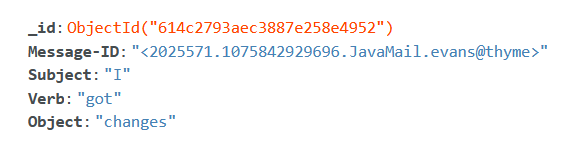
\includegraphics[width = 0.9\textwidth]{Imagenes/Bitmap/initexample.png}}%
	\caption{Ejemplo de documento de un Information Item}%
	\label{fig:initexample}
\end{figure}

Durante el proceso de almacenamiento, también se ha llevado a cabo un primer filtrado de mensajes que no son de utilidad para el propósito que persigue este trabajo y que, por tanto, pueden ser descartados sin guardarlos en MongoDB. Estos son: los correos electrónicos que carecen de cuerpo (puede ser porque originalmente no poseían o porque tras las operaciones de limpieza del mismo que han sido explicadas en la sección \ref{ss:prep}, se produzca esta situación), los e-mails de los que no se extrae ningún Information Item (ya que los InIts serán la entrada de nuestro sistema de generación de lenguaje natural) y los mensajes que son consecuencia de un error en el servidor de mensajería (por ejemplo, al intentar mandar un e-mail con una dirección de destinatario inexistente el servidor de correo siempre manda un mensaje informando de este error). De esta forma, se detectan 35.110 mensajes sin caracteres en el cuerpo, 121.799 correos electrónicos de los que no se extrae ningún Information Item y 7 e-mails consecuencia de errores en el servidor de mensajería, almacenando 360.485 correos electrónicos en la base de datos de MongoDB acompañados de 3.407.099 Information Items.

\subsection{Análisis exploratorio de los datos}\label{ss:eda}
Tras llevar a cabo las tareas de preparación, limpieza de los datos, procesamiento y almacenamiento, con un filtrado a priori, se pueden observar las distribuciones numéricas del corpus desarrollando un análisis exploratorio de los datos. Este estudio preliminar ofrecerá una descripción acerca de los correos electrónicos y sus Information Items.

El primer, y probablemente más sencillo, parámetro que puede analizarse es el número de palabras de cada correo. Para observar cómo se distribuye esta variable en el conjunto de datos, se han calculado las frecuencias requeridas para generar la figura \ref{fig:distpal}. En ella puede deducirse que, a pesar de poseer correos electrónicos con una gigantesca cantidad de palabras, la mayoría de mensajes muestran un número más considerable para tratarse de e-mails.

\begin{figure}[h]
	\centering%
	\centerline{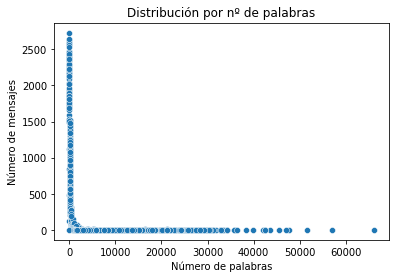
\includegraphics[width = 0.6\textwidth]{Imagenes/Bitmap/dist-palabras.png}}%
	\caption{Distribución del número de palabras en los mensajes}%
	\label{fig:distpal}
\end{figure}
